\chapter{定理证明的可视化}
在数理逻辑领域,一个逻辑公式的形式化证明通常被表示成一个公式序列,其中这个公式序列中的每个公式既可以是公理,也可以是之前公式的逻辑推导结论。一种更加自然的表示公式的形式化证明的方式是将证明表示成一棵树,其中这颗树的每一个节点都用一个公式标记,而该节点的子节点则标记为相应公式的逻辑前提。如今,随着计算机定理证明工具的应用,逻辑公式的形式化证明树可由计算机以自动或者半自动(需要人工干预)的方式生成。然而,目前定理证明工具的输出都是文本格式的,这就使得当证明树的机构较复杂或者节点较多的时候不容易使人理解。同样的问题也出现在模型检测领域,当Kripke模型的结构较复杂的时候,文本格式的输出通常无法直观的展示由模型检测工具生成的反例。
另外,在上一章中我们提到,\sctlprov{}在验证Kripke模型的性质的时候,相比于传统的模型检测工具,能生成更丰富的验证结果。\couic{而且,在传统的模型检测工具和定理证明工具中,验证的结果通常是以文本形式输出的,而文本形式的输出通常无法清晰地表达对于结构复杂的Kripke模型的状态搜索,也无法完整展现模态词嵌套的公式的证明树。}为了能将\sctlprov{}的证明输出结果以及证明过程得以清晰并完整的展现出来,在本章我们介绍\tool{VMDV}\footnote{\url{https://github.com/terminatorlxj/VMDV}}(Visualization for Modeling, Demonstration and Verification)。

\tool{VMDV}是一个将证明树及其他数据结构(比如Kripke模型)在3D空间内进行动态可视化布局和显示的工具。相比于其他的证明可视化工具,\tool{VMDV}具有四个特点:
\begin{enumerate}
	\item 目前大多数的证明可视化工具\cite{byrnes2009visualizing,LibalRR14,sakurai2011mikibeta,steel2005visualising}都使用2D图形来完成证明树的绘制,并且可以用不同的颜色来区分证明树中不同的分支或节点。不同于这些工具,\tool{VMDV}是在3D空间中实现证明树的绘制,除了具备2D图形相比文本格式更直观的优点之外,3D空间相比2D空间可以容纳更多的节点和更复杂的图形结构,从而在展示大型证明树时更有优势。
	\item 另一方面,除了\tool{VMDV}之外,目前也有其他可在3D空间内实现证明树绘制的工具\cite{Farmer200939,bajaj2003interactive}。然而,目前的3D证明可视化工具的布局算法是比较原始的,当在这些工具中展示较多的节点时,所有的节点往往按照一个或若干个既定的方向做延伸状排列,这种布局方式使得3D图形的展示既不美观,又降低了空间利用率。不同于这些工具,\tool{VMDV}利用动态布局算法,将所有的节点看作是相互之间具有斥力的物体,而连接节点之间的边则可看作是具有引力的弹簧,通过每个节点所受的引力和斥力来随时更新节点在3D空间内的位置,并在整个布局过程中随时更新节点间的引力和斥力,直到所有节点的受力达到平衡状态。整个证明树就可看作一个自适应的物理系统,由此得出的节点布局更自然美观,也能充分填充3D空间。
	\item 在传统的具有人工干预的定理证明工具(比如Coq\footnote{\url{https://coq.inria.fr/}})中,证明树的节点通常随时被加入或者删除。\tool{VMDV}可实现证明树结构的动态更新的可视化。
	\item 不同于传统的证明可视化工具通常只针对于一种定理证明工具的输出的可视化,我们在\tool{VMDV}中定义了可与不同的定理证明工具的接口\footnote{\url{https://github.com/terminatorlxj/VMDV/blob/master/protocol.md}}。实现这个接口的定理证明工具或者其插件都可以利用\tool{VMDV}的功能来实现证明的可视化。
\end{enumerate}


\tool{VMDV}利用\textsf{OpenGL}的绘图接口来编写显示引擎,并用Java编程语言来实现布局算法与其他工具的数据通信。接下来,我们分别介绍\tool{VMDV}的相关技术细节及其应用。

\section{背景知识}
这一小节讲的是有关可视化的相关背景知识。
\subsection{OpenGL}\label{vmdv:opengl}
\textsf{OpenGL},全称Open Graphics Library,是一个跨编程语言并且跨平台的编程接口的标准。在计算机系统中,通常由显卡提供\textsf{OpenGL}的实现。一个典型的基于\textsf{OpenGL}的3D图形的显示过程为:首先,用户程序通过调用\textsf{OpenGL}的绘图\textsf{API}(Application Programming Interface)来定义一组要显示的图形的数据和命令,并将这些数据和命令存储在计算机的主内存(RAM)中;然后,计算机的中央处理器(CPU)会通过CPU时钟将这些数据和命令发送到显卡的显存(VRAM)中,并在图形处理器(GPU)的控制下完成图形的渲染;最后,图形渲染的结果会被存入帧缓冲区中,而帧缓冲区中的帧则最终被发送到计算机的显示器上,并显示出结果。

\subsection{信息可视化}
信息可视化是一个研究如何利用计算机图形学技术将数据中的抽象信息可视化的研究领域。抽象信息的可视化表达可以用来帮助人们揭示数据的隐匿模式,用来帮助更好地理解和发现数据中的规律。得益于计算机图形学理论的日益成熟以及计算机硬件的飞速发展,信息可视化系统能可视化越来越大的数据集以及越来越复杂的数据结构,并在许多行业中发挥着举足轻重的作用。比如,在知识管理领域,信息可视化系统可以用来研究不同学科领域知识之间的关系和演化\cite{ZHHW16};在城市交通系统的研究中,信息可视化系统可以将城市的公共交通工具的卫星定位数据进行可视化,以帮助人们研究和改善公共交通的效率\cite{FYL15}。

\section{\tool{VMDV}的实现}
这一小节讲的是\tool{VMDV}的架构,接口以及3D图形的自动布局算法。
\subsection{\tool{VMDV}的架构}
\begin{figure}[!h]
	\scriptsize
	%\vspace{2.5cm}
	\centering
	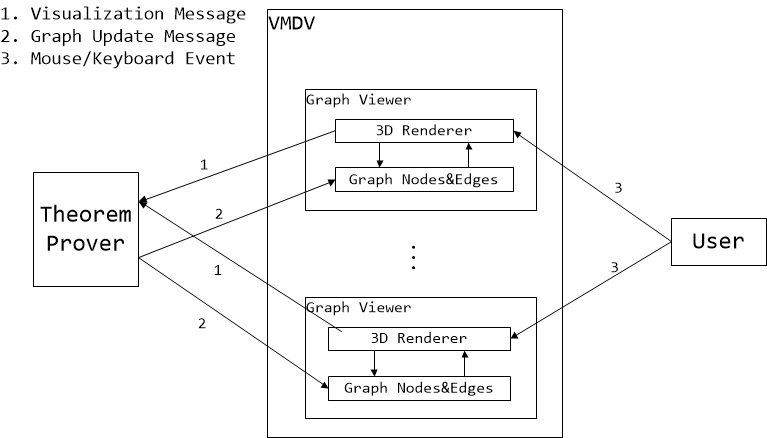
\includegraphics[width=12cm]{./Img/architecture.png}
	\caption{\textsf{VMDV}的架构}
	%\vspace{-10pt}
	\label{fig:architecture}
\end{figure}
如图\ref{fig:architecture}所示,\tool{VMDV}可同时在多个程序窗口中显示3D图像,在\tool{VMDV}中,每个程序窗口都分别包含一个3D渲染器和一个由多个点和边组成的图。3D渲染器的作用是读入图中的点和边的信息,然后根据布局算法确定点和边的位置,最后在3D空间中将图渲染出来。其中,图中的点和边可以通过接收定理证明器传递的消息来动态的添加、删除以及更改,同时3D渲染器对图的更改进行动态的显示,然后向定理证明器发送反馈消息。在3D渲染器工作的同时,\tool{VMDV}同样接收用户传递的交互消息(键盘或鼠标消息),并及时地在3D渲染器中做出反应。

可以看出,\tool{VMDV}同时可以接收两种消息:定理证明器传递过来的消息以及用户给定的消息。其中,定理证明器的消息是以\textsf{TCP}数据包的形式传输的。因此,定理证明器与\tool{VMDV}在网络上通过给定的通讯接口进行交互,而不一定在同一机器上甚至同一进程中。这种设计方式大大减少了\tool{VMDV}对特定的定理证明器的依赖。用户通过传递给\tool{VMDV}消息,可是实现对3D图像的操作:旋转、放大、缩小、高亮、搜索以及触发自定义操作。通过这两种消息,\tool{VMDV}可以实现与定理证明器和用户的交互。

下面我们分别介绍\tool{VMDV}与定理证明器和用户的交互。
\subsection{\tool{VMDV}与定理证明器的交互}
上面我们说到,\tool{VMDV}与定理证明器的交互是通过\textsf{TCP}数据包形式的消息传递来实现的。其中,每个\textsf{TCP}数据包都包含一个\textsf{JSON}格式的数据结构,不同的\textsf{JSON}数据结构可被解析为两种类型的消息:控制消息和反馈消息。

首先,我们介绍控制消息:
\begin{itemize}
	\item \textbf{初始化显示窗口}({定理证明器} $\longrightarrow$ \tool{VMDV}):在\tool{VMDV}中,我们将每个显示窗口成为一个会话(Session)。当定理证明器需要可视化一个数据结构(比如证明树)的时候,定理证明器发送一个“create\_session”消息, 指定需要可视化的数据结构的名称(“session\_id”)、简介(“session\_descr”)及类型(“graph\_type”)。其中,定理证明器指定的可视化的数据结构的类型分为两种:树(“Tree”)和有向图(“DiGraph”),前者通常用来表示证明树,后者通常用来表示可能有环的有向图。\tool{VMDV}接收到该消息之后立即初始化并显示一个窗口,并等待定理证明器的进一步消息。
	\begin{verbatim}
	{
	  "type": "create_session",
	  "session_id": string,
	  "session_descr": string,
	  "graph_type": string
	}
	\end{verbatim}
	\item \textbf{添加节点}(定理证明器 $\longrightarrow$ \tool{VMDV}):向\tool{VMDV}相应的会话中加入一个节点,并指定节点的标识(“id”)、要显示的字符串(“label”)、状态(“state”)。其中,节点的状态分为两种:已证明(“Proved”)和未证明(“Not\_Proved”),不同状态的节点通常用不同的颜色高亮显示。\couic{已证明的节点通常默认高亮为绿色,而未证明的节点通常默认高亮为黄色。}
	\begin{verbatim}
	{
	  "type": "add_node",
	  "session_id": string,
	  "node":
	    {
	      "id": string,
	      "label": string,
	      "state": string
	    }
	}
	\end{verbatim}
	\item \textbf{删除节点}(定理证明器 $\longrightarrow$ \tool{VMDV}):在指定的会话中删除一个指定的节点。
	\begin{verbatim}
	{
	  "type": "remove_node",
	  "session_id": string,
	  "node_id": string
	}
	\end{verbatim}
	\item \textbf{添加边}(定理证明器 $\longrightarrow$ \tool{VMDV}):在指定的会话中添加一条由“from\_id”节点指向“to\_id”节点的边,同时指定该条边上要显示的字符串(“label”)。
	\begin{verbatim}
	{
	  "type": "add_edge",
	  "session_id": string,
	  "from_id": string,
	  "to_id": string,
	  "label": string
	}
	\end{verbatim}
	\item \textbf{删除边}(定理证明器 $\longrightarrow$ \tool{VMDV}):在指定的会话中删除由“from\_id”节点指向“to\_id”节点的边。
	\begin{verbatim}
	{
	  "type": "remove_node",
	  "session_id": string,
	  "node_id": string
	}
	\end{verbatim}
	\item \textbf{高亮节点}(定理证明器 $\longleftrightarrow$ \tool{VMDV}):高亮节点消息可由定理证明器和\tool{VMDV}互相发送给对方。当定理证明器向\tool{VMDV}发送该消息时,\tool{VMDV}在相应的会话中将指定的节点用不同于节点当前的颜色高亮显示。当用户在\tool{VMDV}窗口中执行鼠标选中或者搜索操作时,被选中或者搜索到的节点在窗口中被高亮显示的同时,将所有节点的高亮消息发送到定理证明器。当定理证明器同时在\tool{VMDV}中可视化多个数据结构时,高亮节点消息的传递过程可用来实现多个数据结构的交互显示。比如,在可视化\sctlprov{}的证明结果的时候,\tool{VMDV}通常会初始化两个窗口,分别可视化当前公式的证明树,以及在搜索当前证明树的过程中所访问到的Kripke模型的状态。当用鼠标选中或搜索到证明树的某个或某些节点时,\tool{VMDV}将这些证明树节点的高亮信息发送给\sctlprov{},同时\sctlprov{}识别相应的证明树节点,并计算出与这些证明树节点相关的状态,然后将这些状态节点的高亮信息发送给\tool{VMDV},于是\tool{VMDV}在状态图窗口中高亮显示相应的状态。
	
%	在指定的会话中删除由“from\_id”节点指向“to\_id”节点的边。
	\begin{verbatim}
	{
	  "type": "remove_node",
	  "session_id": string,
	  "node_id": string
	}
	\end{verbatim}
	\item \textbf{取消高亮节点}(定理证明器 $\longleftrightarrow$ \tool{VMDV}):同高亮节点消息一样,取消高亮节点的消息同样可由定理证明器和\tool{VMDV}互相发送给对方。
	\begin{verbatim}
	{
	  "type": "unhighlight_node",
	  "session_id": string,
	  "node_id": string
	}
	\end{verbatim}
	\item \textbf{取消所有高亮}(定理证明器 $\longleftrightarrow$ \tool{VMDV}):去掉所有节点的高亮颜色。
	\begin{verbatim}
	{
	  "type": "clear_color",
	  "session_id": string
	}
	\end{verbatim}
	\item \textbf{删除会话} (定理证明器 $\longrightarrow$ \tool{VMDV}):\tool{VMDV}收到删除会话消息后,销毁对应的窗口,结束一个数据结构的可视化过程。
	\begin{verbatim}
	{
	  "type": "remove_session",
	  "session_id": string
	}
	\end{verbatim}
\end{itemize}

当定理证明器或\tool{VMDV}收到对方发来的控制消息后,会发送回对方一个反馈消息,用来表明该控制消息是否被成功解析:
\begin{itemize}
	\item \textsf{成功解析}(定理证明器 $\longleftrightarrow$ \tool{VMDV}):
	\begin{verbatim}
	{
	  "type": "feedback",
	  "session_id": string,
	  "status": "OK"
	}
	\end{verbatim}
	\item \textbf{解析失败}(定理证明器 $\longleftrightarrow$ \tool{VMDV}):
	\begin{verbatim}
	{
	  "type": "feedback",
	  "session_id": string,
	  "status": "Fail",
	  "error_msg": string
	}
	\end{verbatim}
\end{itemize}
\subsection{\tool{VMDV}与用户的交互}


\subsection{\tool{VMDV}中3D图形的动态布局算法}

\section{\tool{VMDV}的应用}


